\documentclass{beamer}

\usetheme{Boadilla}
\usepackage{polski}
\usepackage{times}
\usepackage[T1]{fontenc}
\usepackage{graphicx}
\usepackage{listings}
\usefonttheme{serif}

\title{Seminarium dyplomowe}
\subtitle{Układ aktywnego tłumienia hałasu pod nadzorem jądra systemu Linux z rozszerzeniami real-time}

\author{Daniel Kopiecki}
\institute{Politechnika Śląska}
\date{\today}

\begin{document}

\begin{frame}
\titlepage
\end{frame}

\begin{frame}
\frametitle{Część sprzętowa}
\framesubtitle{Uproszczony schemat architektury}
\begin{figure}[H]
\centering
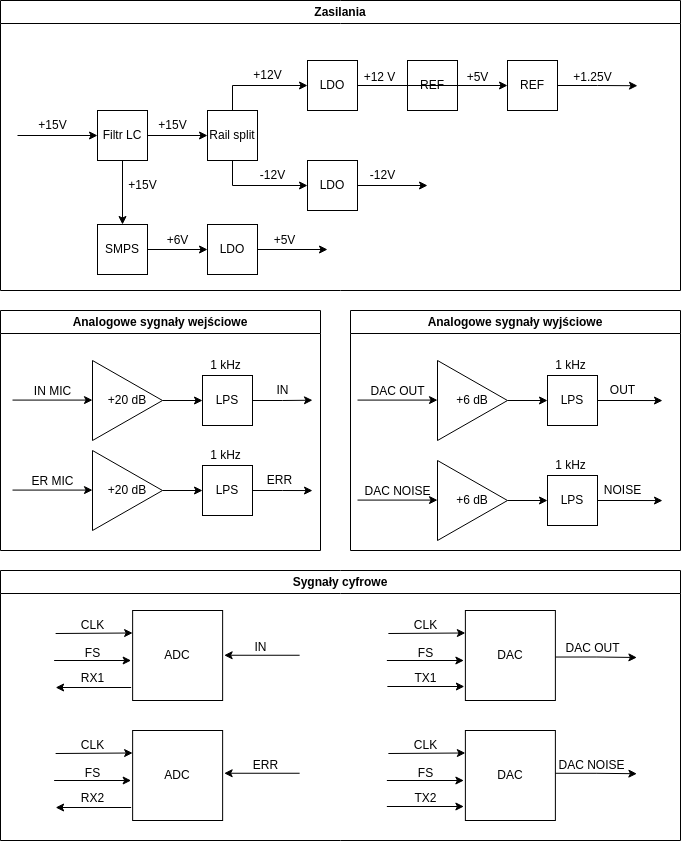
\includegraphics[width=0.4\linewidth]{images/arch.png}
\caption{Architektura sprzętowa}
\end{figure}
\end{frame}

\begin{frame}
\frametitle{Część sprzętowa}
\framesubtitle{Warstwa przednia}

\begin{figure}[H]
\centering
\begin{minipage}{.4\textwidth}
  \centering
  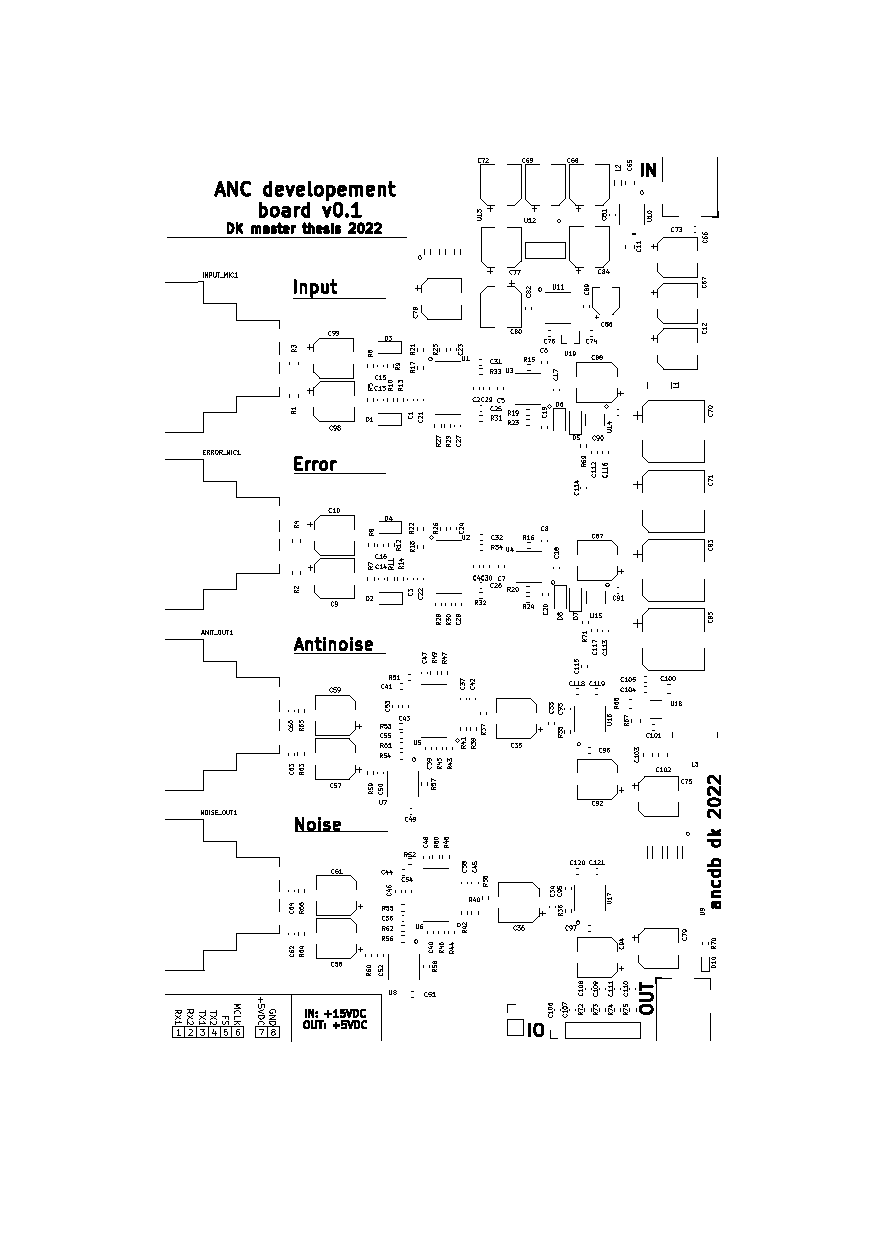
\includegraphics[width=\linewidth]{pdfs/main-F_Silkscreen.pdf}
\end{minipage}%
\begin{minipage}{.4\textwidth}
  \centering
  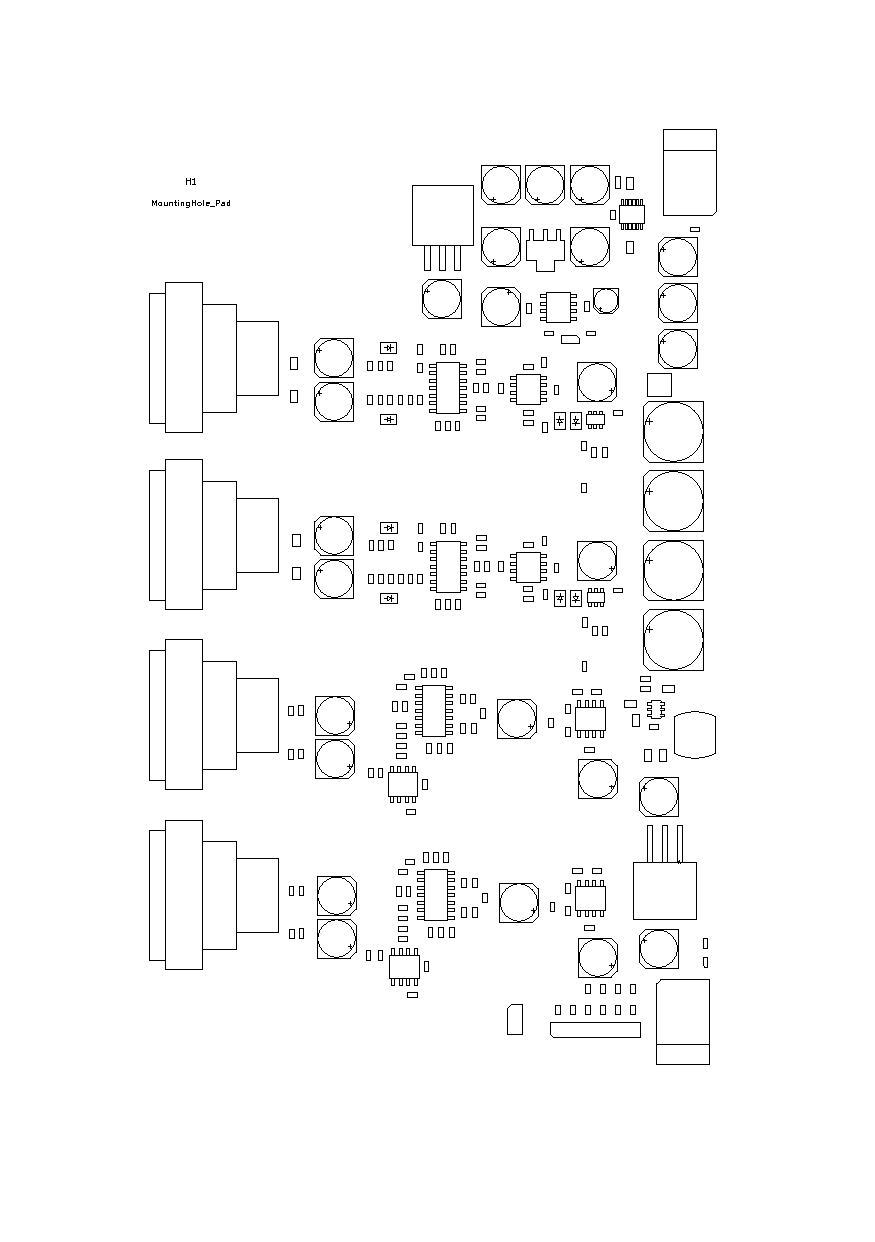
\includegraphics[width=\linewidth]{pdfs/main-F_Fab.pdf}
\end{minipage}
\caption{Warstwa przednia, 1}
\end{figure}

\end{frame}

\begin{frame}
\frametitle{Część sprzętowa}
\framesubtitle{Warstwa przednia}

\begin{figure}[H]
\centering
\begin{minipage}{.4\textwidth}
  \centering
  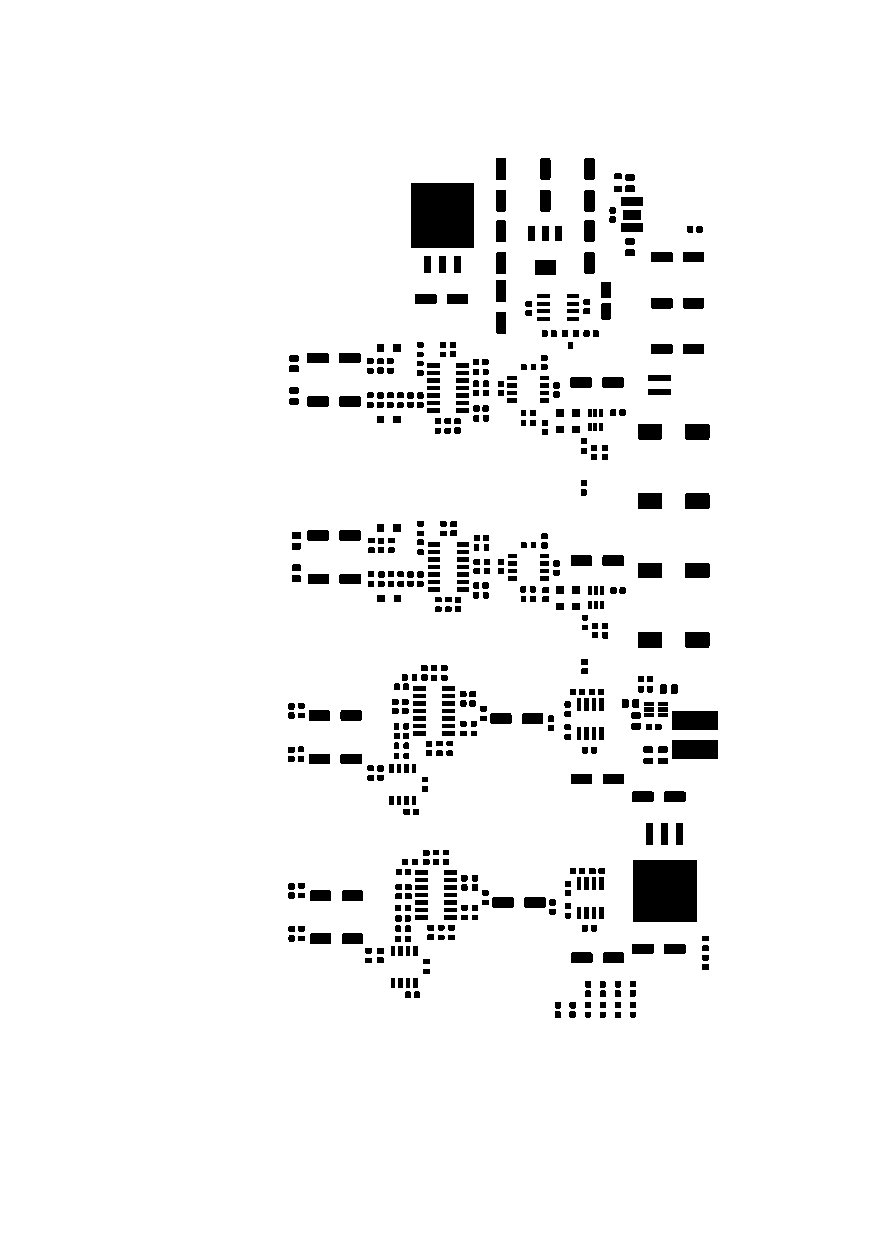
\includegraphics[width=\linewidth]{pdfs/main-F_Paste.pdf}
\end{minipage}%
\begin{minipage}{.4\textwidth}
  \centering
  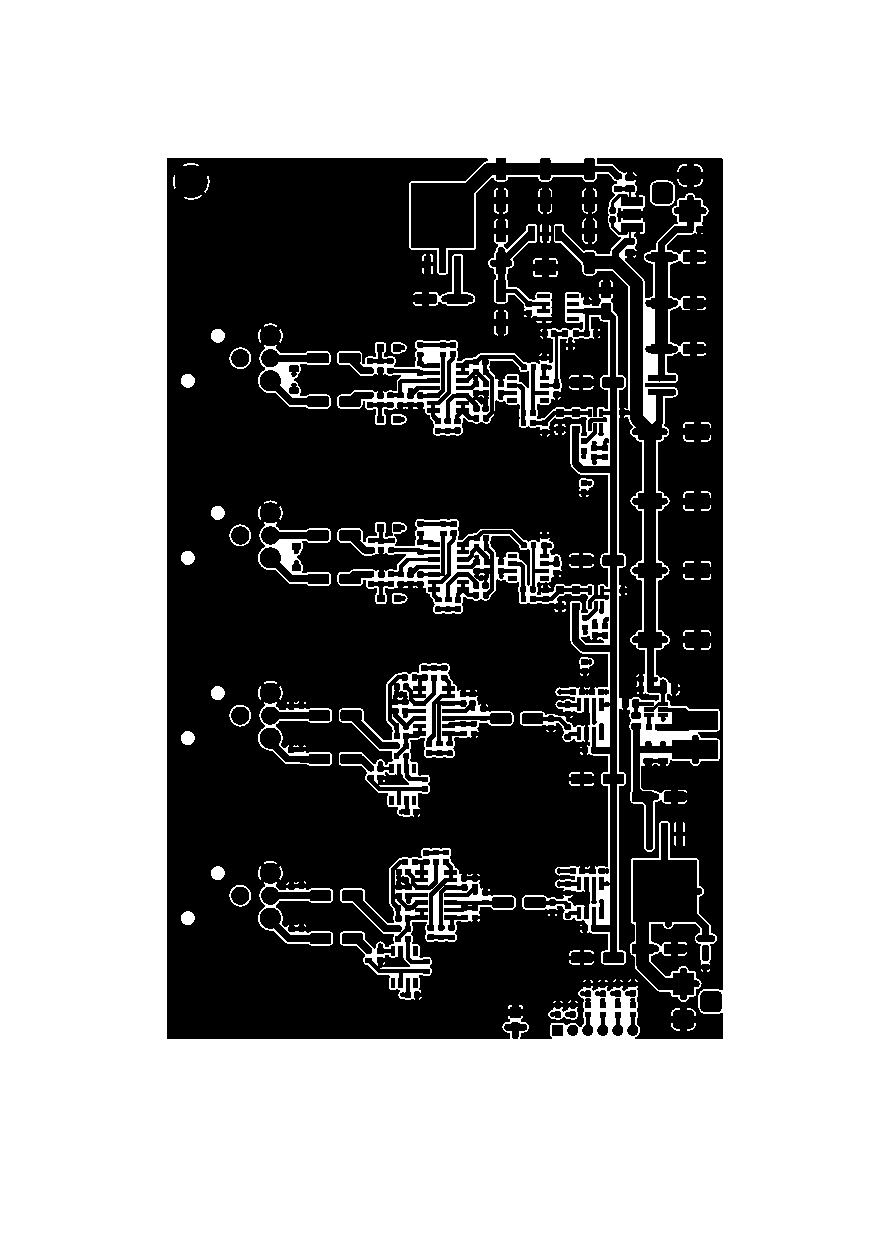
\includegraphics[width=\linewidth]{pdfs/main-F_Cu.pdf}
\end{minipage}
\caption{Warstwa przednia, 2}
\end{figure}

\end{frame}

\begin{frame}
\frametitle{Część sprzętowa}
\framesubtitle{Warstwy środkowe}

\begin{figure}[H]
\begin{minipage}{.4\textwidth}
  \centering
  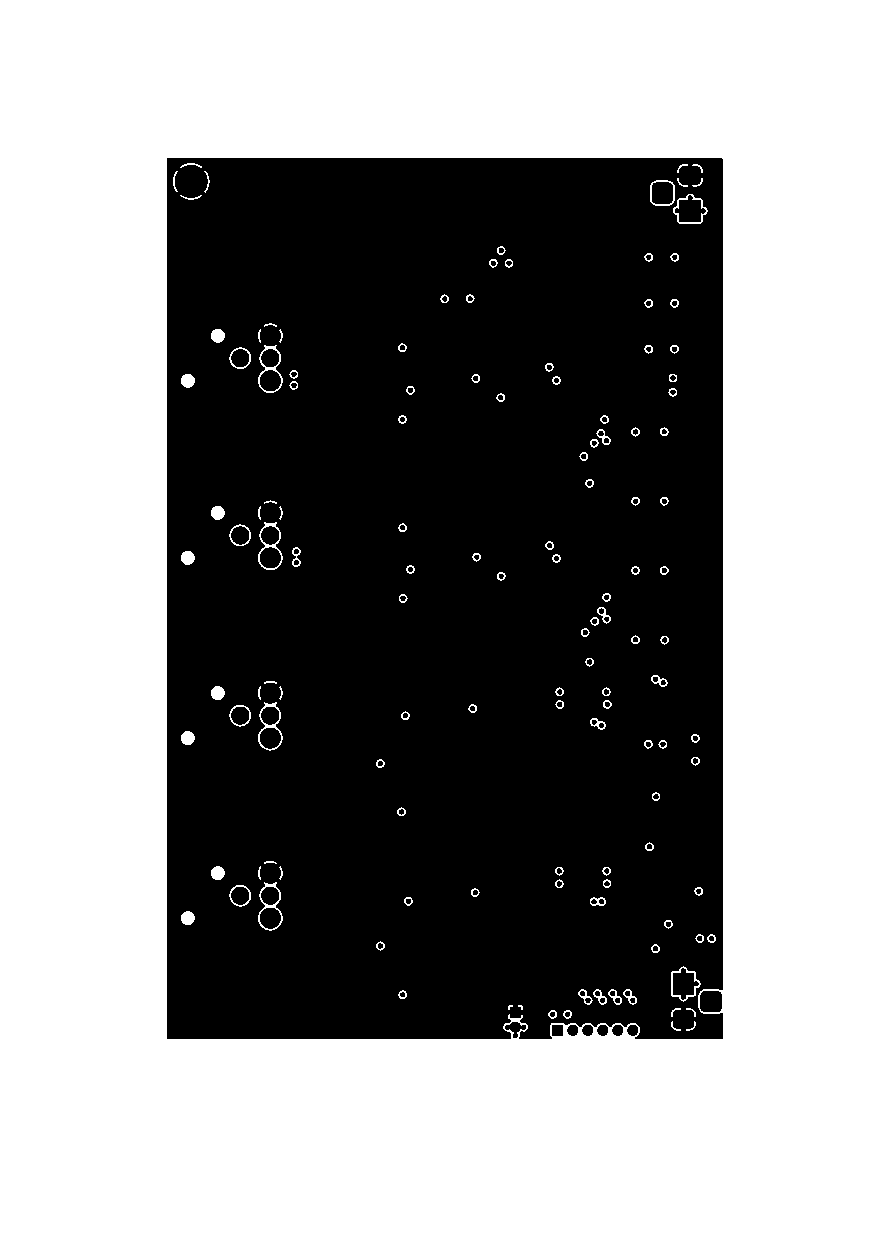
\includegraphics[width=\linewidth]{pdfs/main-In1_Cu.pdf}
\end{minipage}%
\begin{minipage}{.4\textwidth}
  \centering
  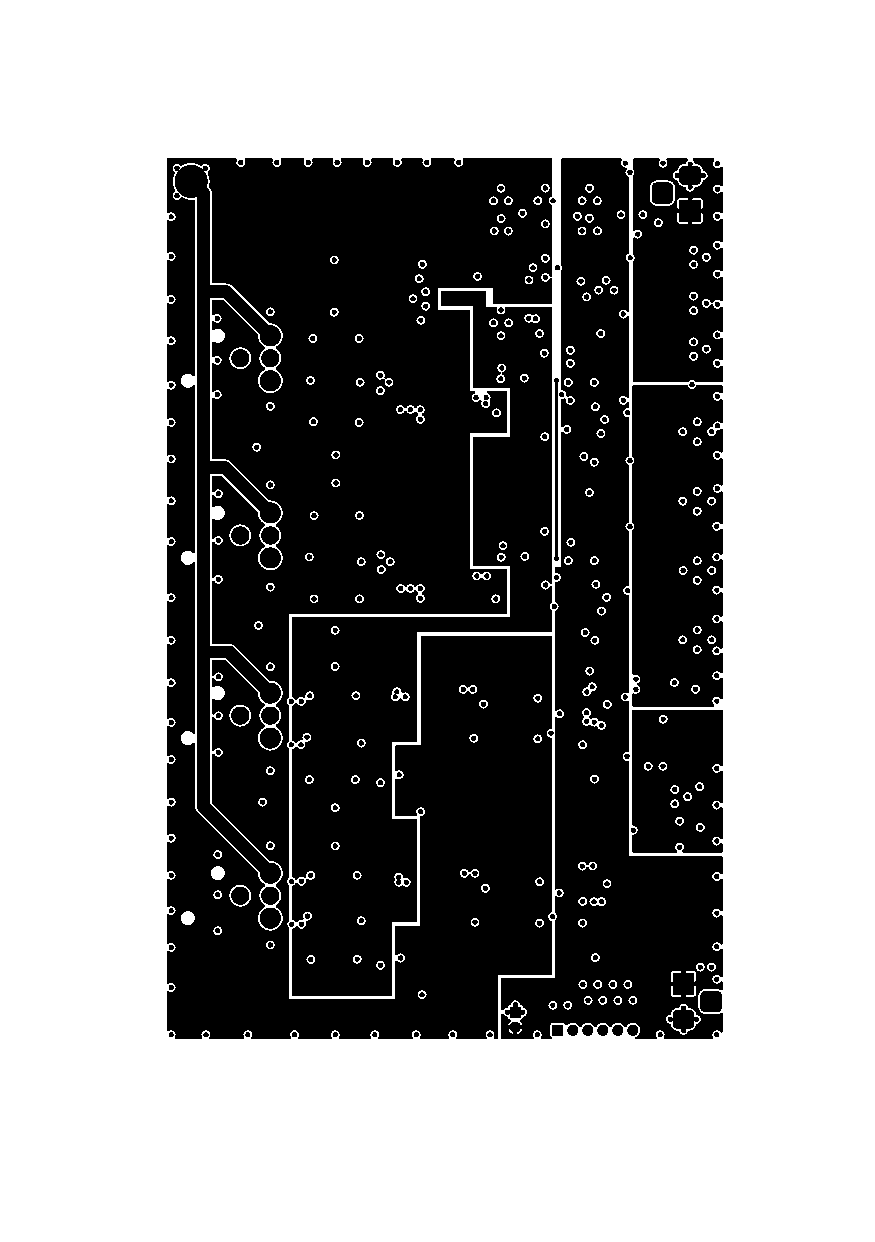
\includegraphics[width=\linewidth]{pdfs/main-In2_Cu.pdf}
\end{minipage}
\caption{Warstwy środkowe}
\end{figure}

\end{frame}

\begin{frame}
\frametitle{Część sprzętowa}
\framesubtitle{Warstwa dolna}

\begin{figure}[H]
\begin{minipage}{.4\textwidth}
  \centering
  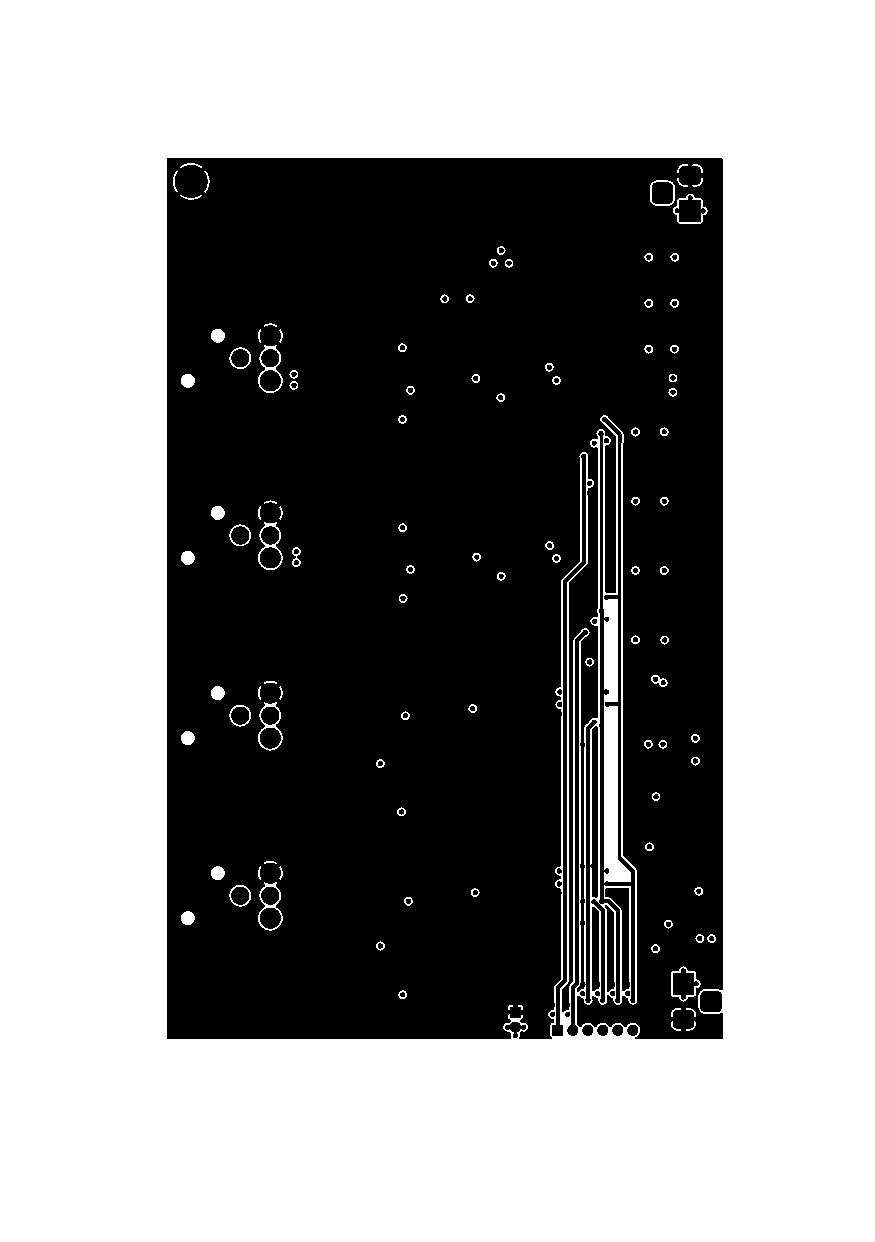
\includegraphics[width=\linewidth]{pdfs/main-B_Cu.pdf}
\end{minipage}%
\begin{minipage}{.4\textwidth}
  \centering
  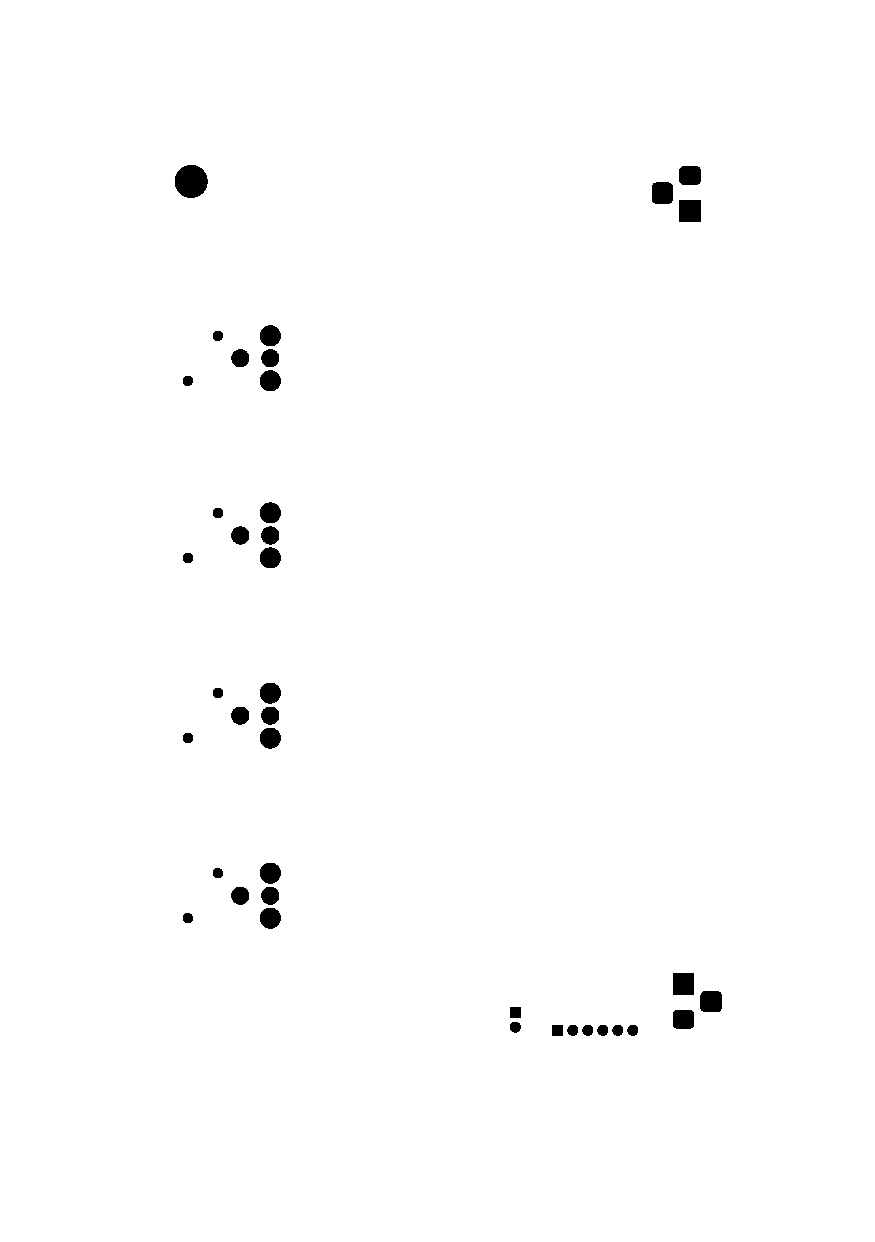
\includegraphics[width=\linewidth]{pdfs/main-B_Mask.pdf}
\end{minipage}
\caption{Warstwa dolna}
\end{figure}
\end{frame}

\begin{frame}
\frametitle{Część sprzętowa}
\framesubtitle{Kilka ciekawych kwestii implementacyjnych}
\begin{itemize}
\item Wszystko wpływa na wszystko
\item Odległość pomiędzy ścieżkami ma \textbf{kolosalne znaczenie}
\item Kwestie obligatoryjne - rozłożenie warst (\textit{stackup}) oraz umiejscowienie komponentów
\end{itemize}
\begin{figure}[H]
\centering
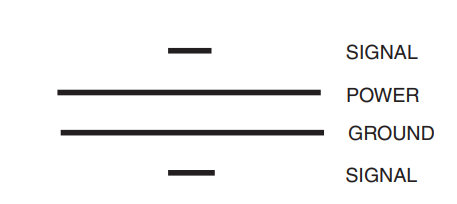
\includegraphics[width=0.5\linewidth]{images/stackup.png}
\end{figure}
\end{frame}

\begin{frame}
\frametitle{Część sprzętowa}
\framesubtitle{Kilka ciekawych kwestii implementacyjnych}
\begin{itemize}
\item Płaszczyzną odniesienia dla relatywnie szybkich sygnałów cyfrowych może w równym stopniu być płaszczyzna masy, jak i płaszczyzna \textbf{zasilania}
\item Z Henry W. Ott, \textit{Electromagnetic Compatibility Engineering} - układ scalony \textbf{nie jest źródłem prądu} sam w sobie, lecz stanowi jedynie jego \textbf{sterownik}. Prawdziwym źródłem jest kondensator odsprzęgający lub/i pasożytnicza pojemność pomiędzy ścieżkami/płaszczyznami.
end{frame}
\end{itemize}
\begin{figure}[H]
\centering
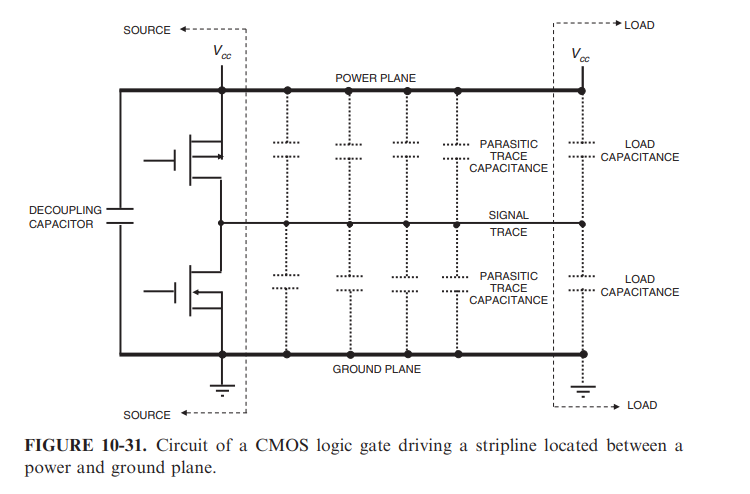
\includegraphics[width=0.4\linewidth]{images/l_current_flow.png}
\caption{Możliwe drogi sygnałów cyfrowych}
\end{figure}
\end{frame}


\begin{frame}
\frametitle{Część sprzętowa}
\framesubtitle{Wykorzystywany protokół cyfrowy}
\begin{itemize}
\item Bardzo ważną kwestią implementacyjną jest opracowanie synchronicznego próbkowania wszystkich przetworników. Aby to uzyskać, konieczny jest protokół cyfrowy, który zapewni zegar, odpowiednią manipulację selektorem, dwie linie RX oraz dwie linie TX.
\end{itemize}
\begin{figure}[H]
\centering
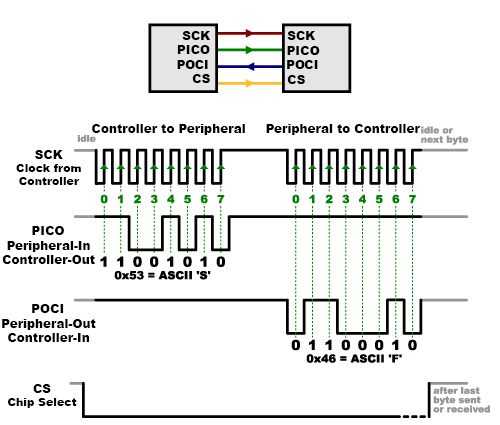
\includegraphics[width=0.4\linewidth]{images/spi.png}
\caption{Protokół SPI - \textit{Serial Peripheral Interface}}
\end{figure}

\end{frame}

\begin{frame}
\frametitle{Część sprzętowa}
\framesubtitle{Protokół cyfrowy - możliwe rozwiązania}
\begin{itemize}
\item McASP - protokół cyfrowy opracowany przez Texas Instruments w celu interakcji z wielokanałowymi kartami dźwiękowymi - podejście \textbf{optymalne}
\end{itemize}
\begin{figure}[H]
\centering
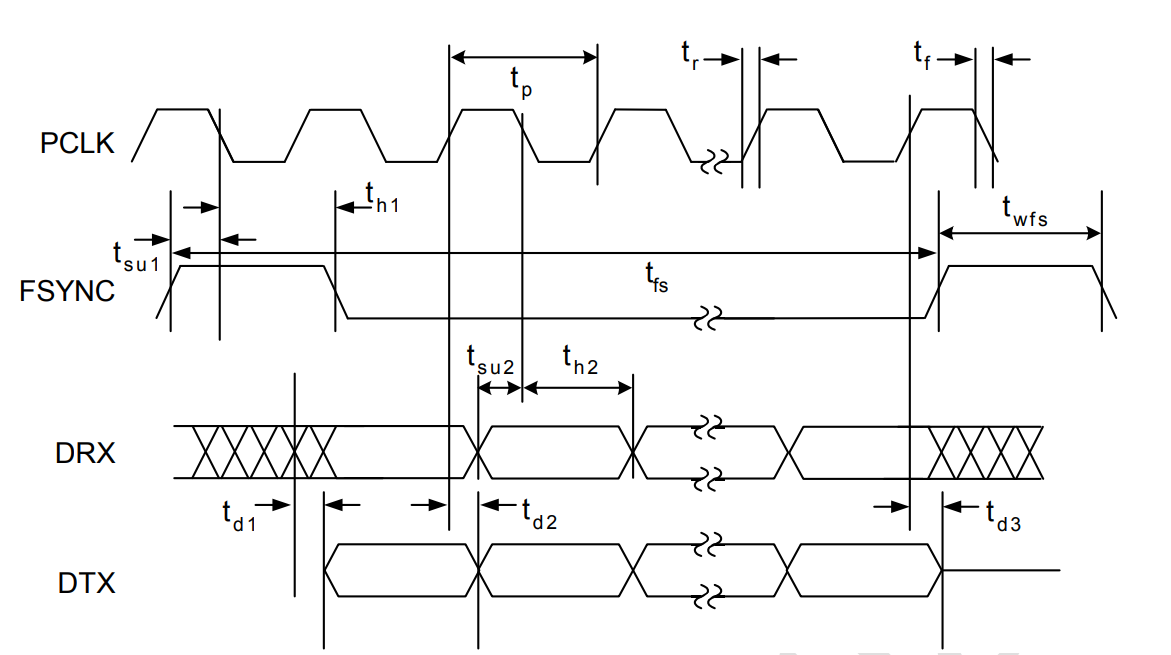
\includegraphics[width=0.5\linewidth]{images/mcasp.png}
\caption{Protokół McASP - \textit{Multichannel Audio Serial Port}}
\end{figure}

\end{frame}

\begin{frame}
\frametitle{Część sprzętowa}
\framesubtitle{Protokół cyfrowy - możliwe rozwiązania}
\begin{itemize}
\item \textit{Bit banging} - metoda transmisji danych oparta na implementacji dedykowanego protokołu cyfrowego z wykorzystaniem dwustanowych pinów wejściowo-wyjściowych (\textit{GPIOs}) - podejście \textbf{ostateczne}. Wymaga implementacji sterownika na najniższym poziomie.
\end{itemize}
\end{frame}

\begin{frame}[fragile]
\frametitle{Część sprzętowo-programowa}
\framesubtitle{Protokół cyfrowy - bit banging, przykład}

\begin{lstlisting}[frame=single, language=C, basicstyle=\tiny]
void tx_byte(uint8_t data)
{
	gpio_low(SD_CS);
	for (uint8_t i = 0u; i < 8u; ++i) {
		if (data & 0x80u)
			gpio_high(SD_DI);
		else
			gpio_low(SD_DI);
		
		gpio_low(SD_CLK);
		delay();
		gpio_high(SD_CLK);
		
		data <<= 1u;
	}
	
	gpio_low(SD_CS);
}
\end{lstlisting}
\end{frame}

\begin{frame}
\frametitle{Część programowa}
\framesubtitle{ALSA}
\begin{itemize}
\item Na chwilę obecną wybrana została ścieżka \textbf{optymalna}.
\item Tak jak pisano wcześniej, protokół McASP wykorzystywany jest do interakcji z kartami dźwiękowymi. 
\item Głównym środowiskiem do interakcji z urządzeniami audio pod systemem operacyjnym GNU/Linux jest \textbf{ALSA} (\textit{Advanced Linux Sound Architecture})

\begin{figure}[H]
\centering
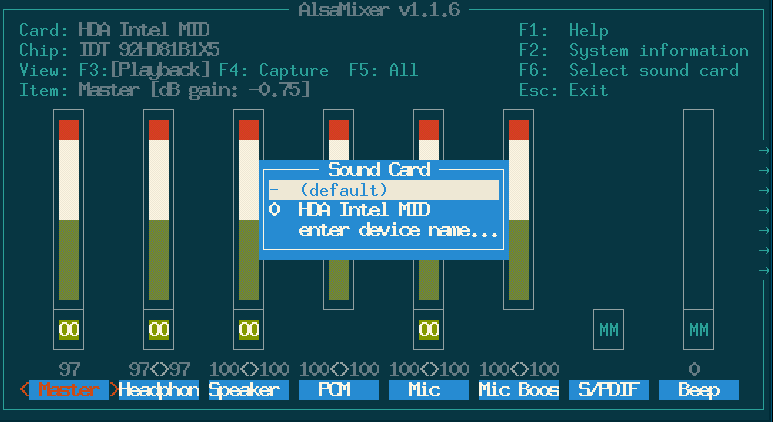
\includegraphics[width=0.5\linewidth]{images/alsamixer.png}
\caption{ALSA - widok aplikacji \textit{AlsaMixer} (\$ alsamixer)}
\end{figure}

\end{itemize}
\end{frame}

\begin{frame}
\frametitle{Część programowa}
\framesubtitle{ALSA}
\begin{itemize}
\item \textbf{ALSA} udostępnia duże, niskopoziomowe API do interakcji z kartami dźwiękowymi z poziomu przestrzeni użytkownika (\textit{userspace}).
\item Plik nagłówkowy biblioteki nosi nazywę \textit{asoundlib.h} a sama biblioteka \textit{libasound}
\end{itemize}

\begin{figure}[H]
\centering
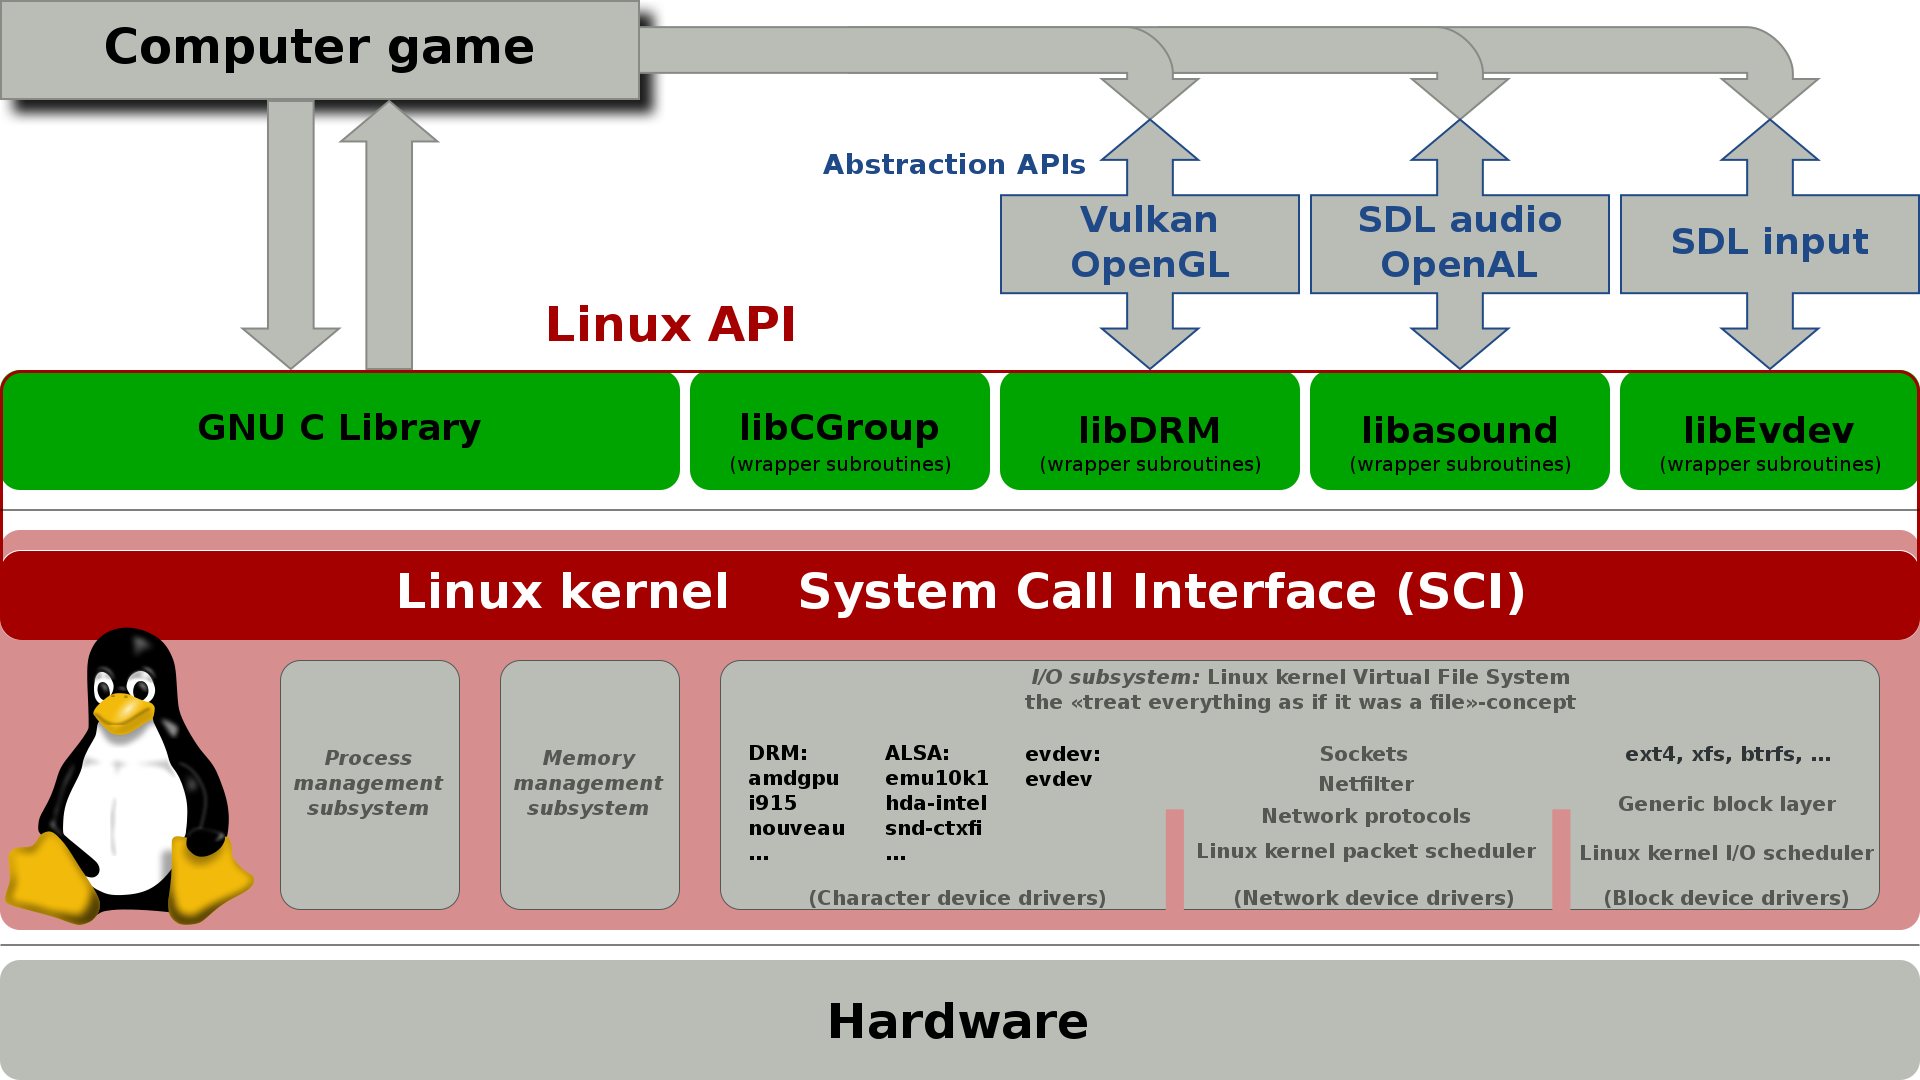
\includegraphics[width=0.8\linewidth]{images/alsa.png}
\caption{Schemat interkacji jądro - przestrzeń użytkownika}
\end{figure}

\end{frame}

\begin{frame}
\frametitle{Część programowa}
\framesubtitle{Cyfrowa reprezentacja dźwięku}
\begin{itemize}
\item Cyfrową reprezentacją dźwięku, wykorzystywaną przez środowisko \textbf{ALSA} jest modulacja pulsowo-kodowa (\textit{PCM - Pulse Code Modulation}

\begin{figure}[H]
\centering
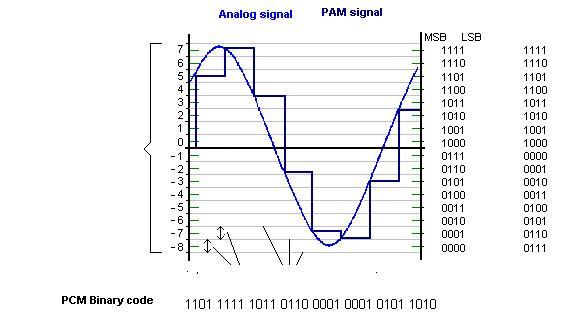
\includegraphics[width=0.8\linewidth]{images/pcm.jpg}
\caption{Modulacja pulsowo-kodowa}
\end{figure}

\end{itemize}

\end{frame}

\end{document}

